\section{FAB-MAP 2.0}

\subsection{Introduction}
\begin{frame}{FAB-MAP 2.0}
    \begin{itemize}
        \item What happened after version 1.0 ?
    \end{itemize}
    \begin{quotation}
        We describe a formulation which preserves almost all the key features of our earlier model, but allows for the exploitation of the sparsity of visual word data to achieve large reductions in computation and memory requirements.~\cite{fabmap2011}
    \end{quotation}
    \begin{itemize}
        \item General intuition of the work in 2.0
            \begin{itemize}
                \item Multiple changes for scalability
            \end{itemize}
    \end{itemize}
\end{frame}

\subsection{Give me a title}
\begin{frame}
    \frametitle{FAB-MAP 2.0}
    \begin{itemize}
        \item Key component: inverted index (did not work out of the box)
        \item They ajusted the likelihood to work with the inverted index (to expensive to compute with negative example)
        \item It deals with negative example to enable inverted index.
        \item Cannot add information of observations of a previously seen scene (only the first observation of the place is taken into account)
        \item Some information lost vs FAB-MAP 1.0

        \item add geometric verification(100 most likely samples) (essential at large scale)... add a figure to show what it is
        \item Pseudocode for the main likelihood calculation required in FAB-MAP is given in Algorithm 1. The complexity of this implementation is O(\#vocab)
        \item validate the work on a 1000km data set; (show the SLAM figure)... Really aimed at large scale (other with 66km but they have the biggest)
    \end{itemize}
\end{frame}

\subsection{K-means}
\begin{frame}{K-Means Modifications}
    \begin{itemize}
        \item Approx algo of k-means
        \item To avoid these effects, we choose the initial cluster centers for k-means using a fixed-radius incremental pre-clustering, where the data points are inspected sequentially, and a new cluster center is initialized for every data point that lies further than a fixed threshold from all existing clus-ters. This is similar to the furthest-first initialization tech-nique (Dasgupta and Long 2005), but more computation-ally tractable for large data sets. (show figure 6,7)
        \item We also modify k-means by adding a cluster merging heuristic. After each k-means iteration, if any two cluster centers are closer than a fixed threshold, one of the two cluster centers is re-initialized to a random location.
        \item This boosted performance of the system
    \end{itemize}
\end{frame}

\begin{frame}{K-Means words}
    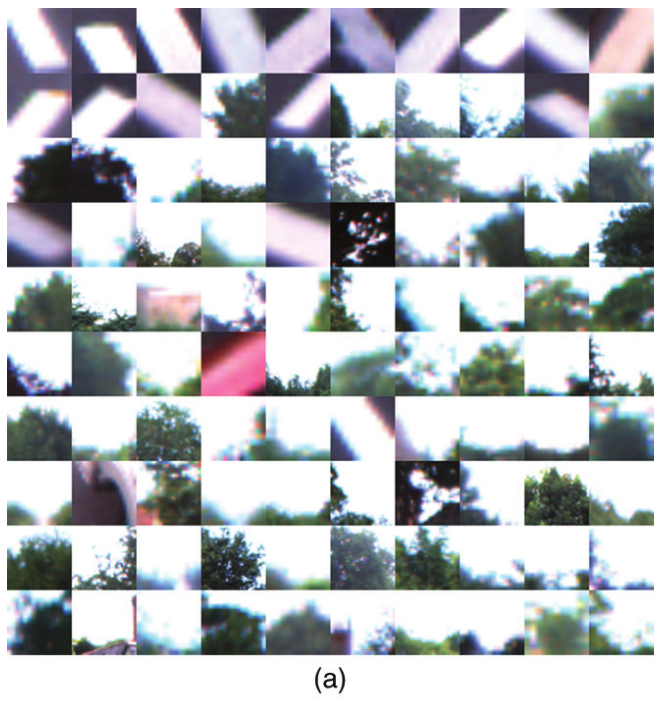
\includegraphics[width=0.5\textwidth]{./media/words_fabmap2a.png}
    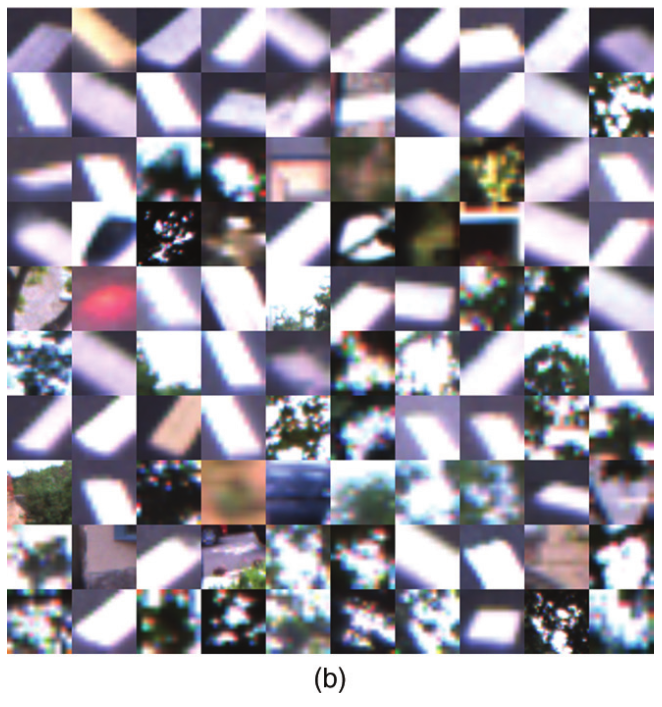
\includegraphics[width=0.5\textwidth]{./media/words_fabmap2b.png}
\end{frame}

\begin{frame}[t]{K-Means Precision-Recall}
    \begin{center}
        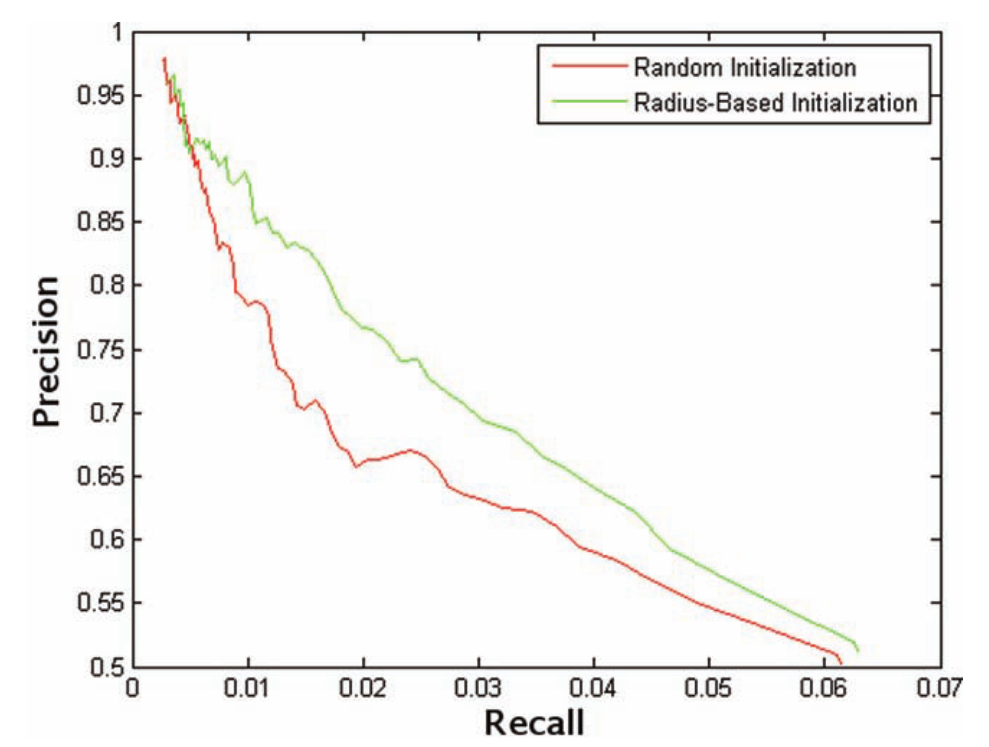
\includegraphics[width=0.7\textwidth]{./media/precision_recall_kmeans.png}
    \end{center}
\end{frame}

\subsection{Results}
\begin{frame}
    \frametitle{Results}
    \begin{itemize}
        \item Ground thruth = GPS, correct match less than 40m... A bit relax (89\% were separated by less than 5 m, and 98\% by less than 10m)
        \item Add result Figure 11
        \item Maybe table 3, indicate that CL vs NB for 100\% precision
        \item 14ms filter update + geo check, 423ms for SURF, 60ms Quantization
        \item 4400 times faster than 1.0, spase representation lead to O(1) instead of O(\#vocab)
    \end{itemize}
\end{frame}

%%%%%%%%%%%%%%%%%%%%%%%%%%%%%%%%%%%%%%%%%%%%%%%%%%%%%%%%%%%%%%%%%%%%%%%%%%%%%%%%

\begin{frame}
    \frametitle{FAB-MAP 2.0}
    At time k, our map of the environment is a collection of nk discrete and disjoint locations Lk = ?L1, ... ,Lnk ?. Each of these locations has an associated appearance model, which we parameterize in terms of unobservable ‘scene elements’, eq. A detector, D, yields visual word observations which are noisy measurements of the existence of the under- lying scene element eq. The appearance model of a location in the map is our belief about the existence of each scene element at that location:
\end{frame}

